\documentclass{acm_proc_article-sp}
\usepackage{verbatim}
\usepackage{graphicx}
\begin{document}

\title{Spectral learning for structured partially observable environments}

\numberofauthors{1}

\author{
\alignauthor
Lucas Langer\\
\email{lucas.langer@mail.mcgill.ca}
}

\date{12 August 2015}

\maketitle

\section{Problem and Motivation}

We consider the problem of learning models of time series data in partially observable environments. Typical applications arise in robotics and reinforcement learning with HMMs and POMDPs being the models of choice. We take  interest in environments with structured observations. Standard learning algorithms are not designed to exploit patterns which arise in many practical applications. As a result, we focus on extending a current learning algorithm to exploit such structure. Our approach yields both better predictive accuracy and computational performance when learning compressed models as one does in practice. 

\section{Background and Related Work}

Predictive state representations are used as a model for computing a probability distribution over observations in a dynamical system. \cite{littman2001predictive}. There exists a well known spectral algorithm which learns a PSR from empirical data \cite{boots2010closing}. The algorithm makes use of Hankel matrices and a singular value decomposition. One can control the number of states in the PSR by only including states with high singular values. The reason for using less states is twofold. First, noise in empirical data artificially creates extra states with low singular values. Secondly, reducing the number of states is necessary in practice for computational performance. 

Learning of PSRs began with the work of \cite{DBLP:conf/icml/Wiewiora05} who used non-spectral methods. Spectral algorithms emerged later and became of interest because they delivered theoretical guarantees far better than other methods. \cite{boots2010closing}. On the applied side spectral learning of PSRs has shown promise in  planning with timing information \cite{pierrelucplanning2015} and in natural language processing for dependency parsing. \cite{balle2013spectral}.

\section{Approach and Uniqueness} 

In our work, we extend the standard PSR learning algorithm by developing a new machinery for performing queries which we call the Base System. The main idea in the Base System is to include transition operators for sequences of observations in addition to those for single observations. We first apply the Base System to timing applications where choosing additional operators is easiest to do. We then progress to the general case of systems with multiple observations and develop a heuristic for choosing effective operators from data.

\section{Results and Contributions}

In the experiments that follow, we produce observations by simulating robot motion in stochastic labyrinth environments. The robot explores the labyrinths until it leaves through one of the doors. We compare PSRs learned with the generic algorithm to PSRs learned with different degrees of the Base System. To measure the performance of a PSR, we compare predictions to the actual probability distribution over observations. Alternatively, one could use cross-validation. 

\subsection{Double Loops}

In the first experiment we look at the time spent in double loop labyrinths. 

%pasted code to include images]

\begin{figure}[ht!]
\centering

\includegraphics[width=60mm]{lucasplots/doubleLoopImage.png}
\caption{Double Loop Environment\label{overflow}}
\end{figure}

\begin{figure}[ht!]
\centering
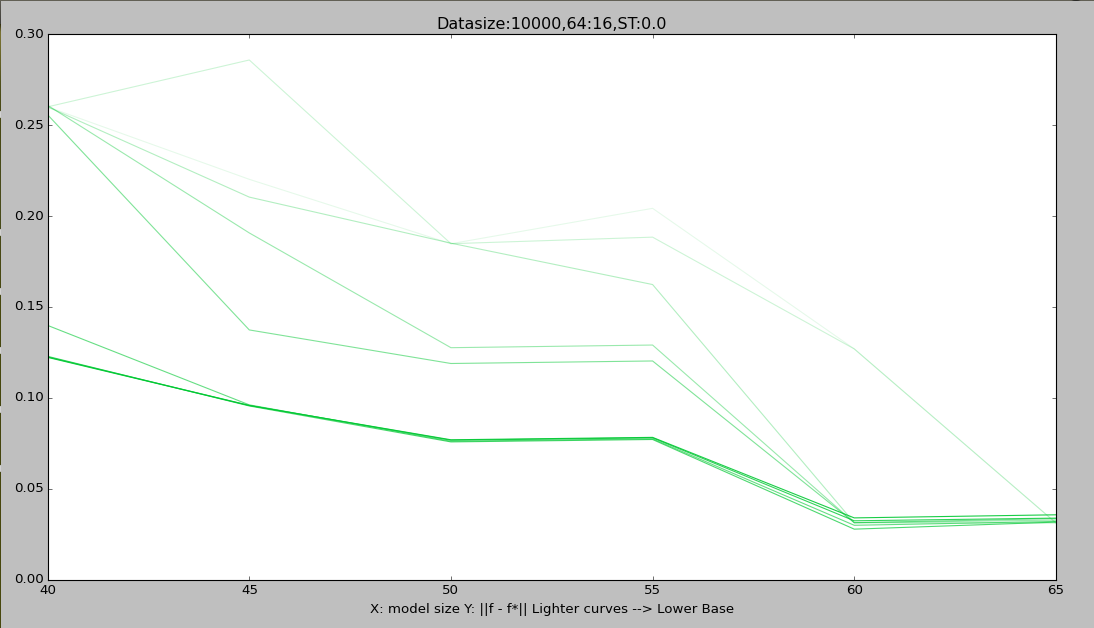
\includegraphics[width=60mm]{lucasplots/doubleloop0.png}
\caption{No noise \label{overflow}}
\end{figure}

%ROBOT INSIDE DOULBE LOOP, GET RID OF SYMMETRY
\begin{figure}[ht!]
\centering
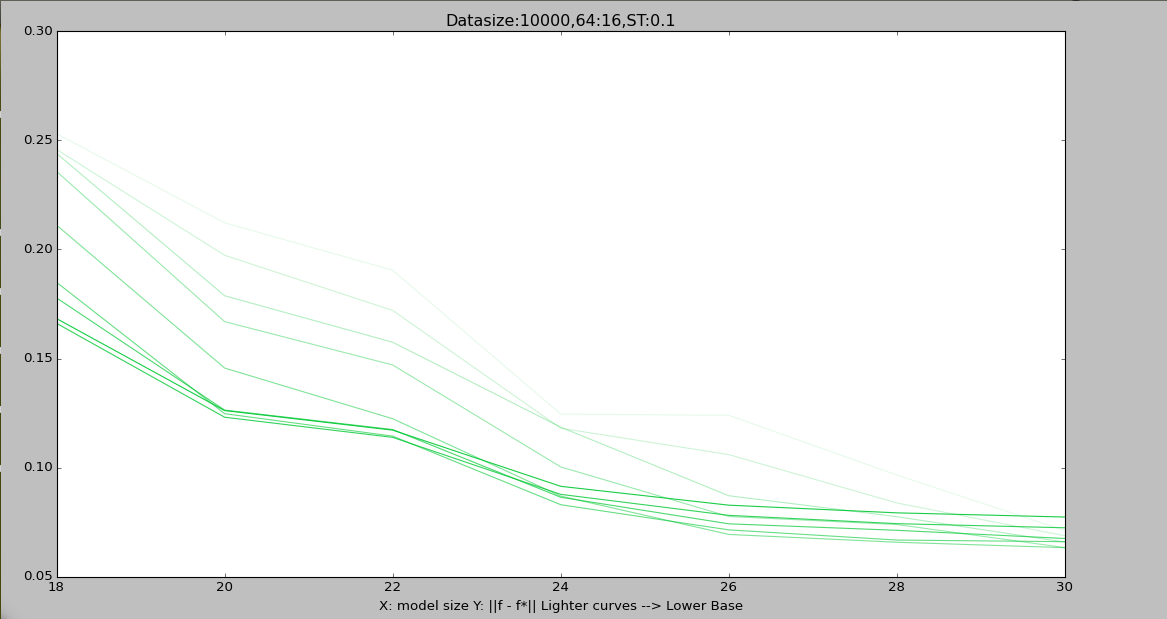
\includegraphics[width=60mm]{lucasplots/doubleloop0_1.png}
\caption{Corridor noise \label{overflow}}
\end{figure}

In both cases, the PSR with the Base System has 100 \% less error than without. In particular, we note that noise in the durations of loops doesn't harm the performance of the Base System.

\subsection{PacMan Labyrinth}

In the second experiment, we look at timing for a PacMan-Type labyrinth. In addition, we use state weightings from the learned PSRs to predict distances between the robot and objects in the environment. 

\begin{figure}[ht!]
\centering
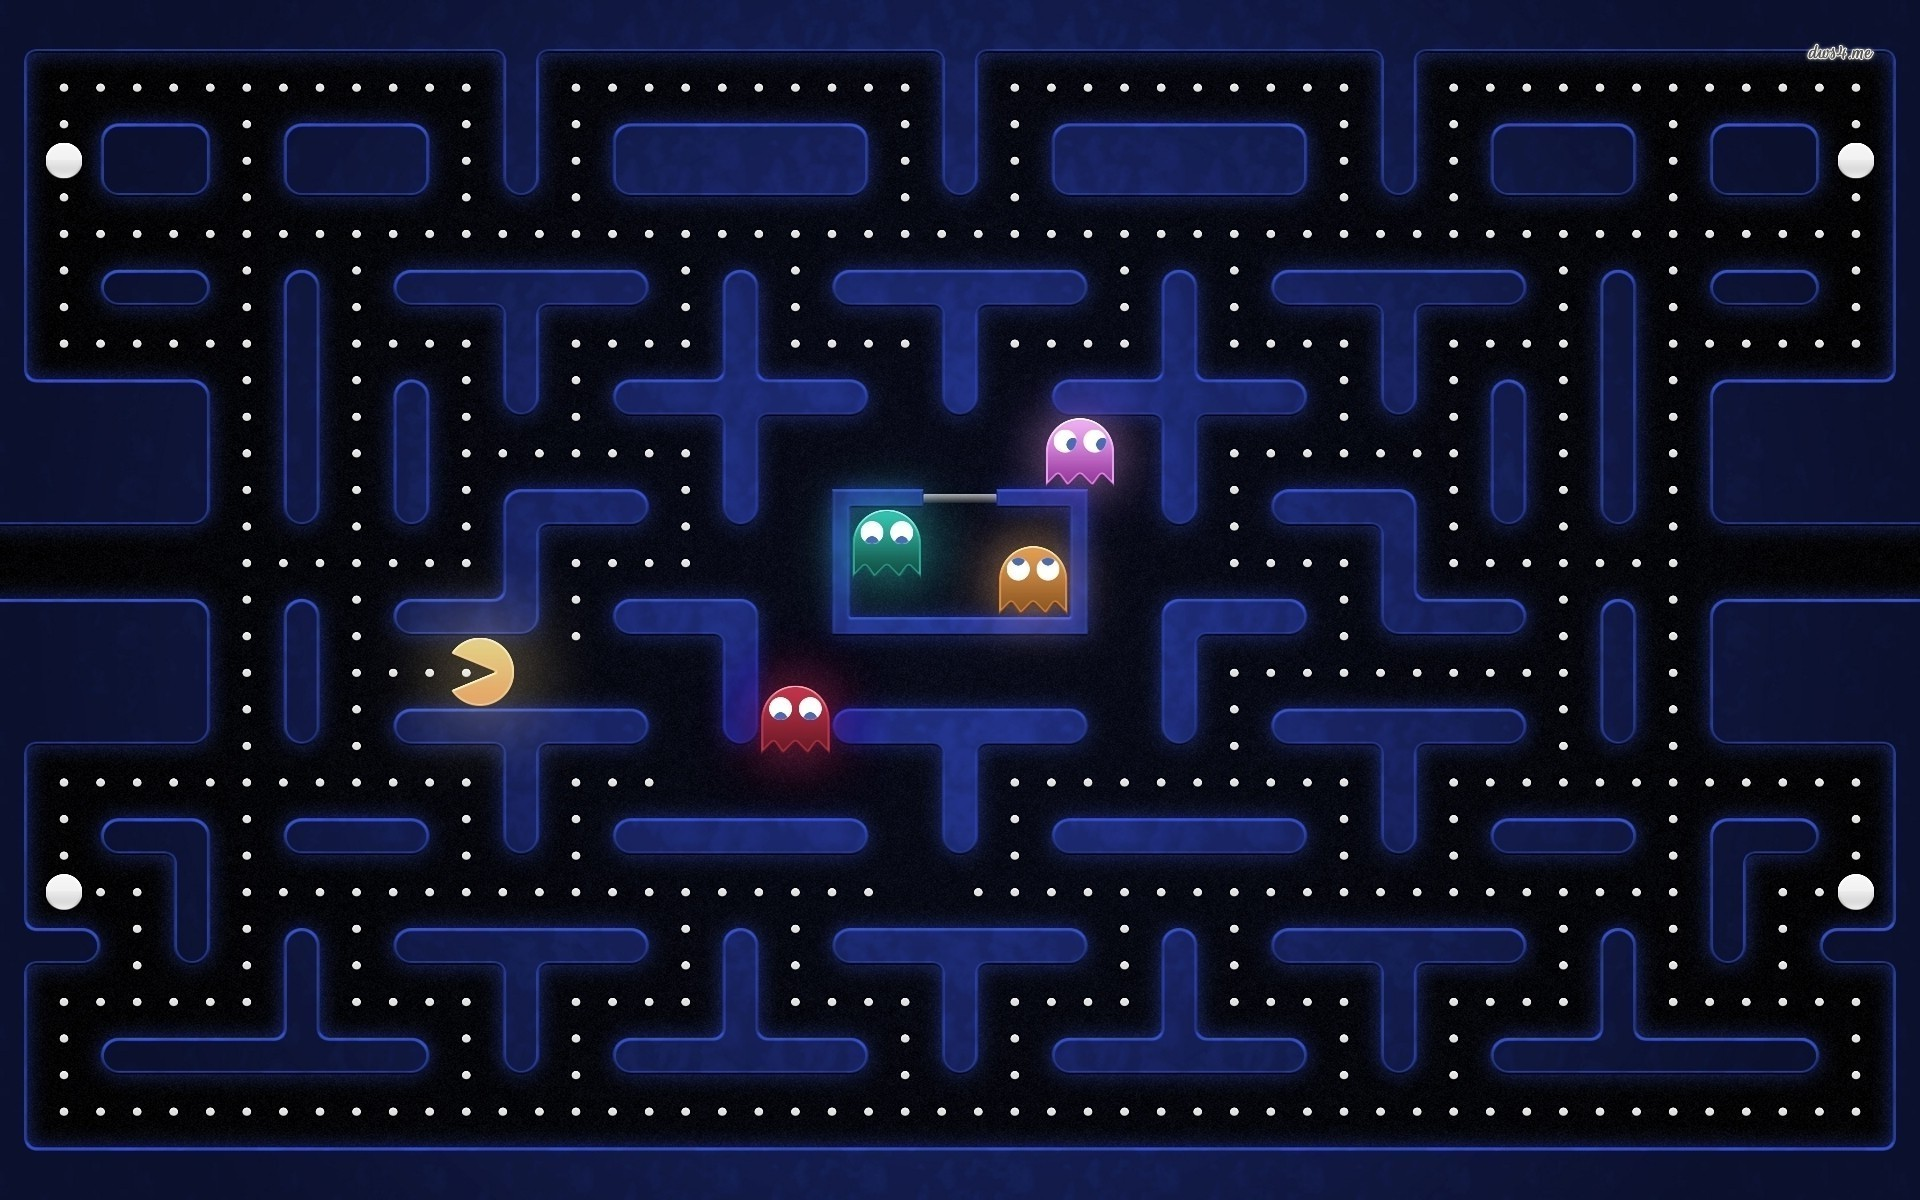
\includegraphics[width=60mm]{lucasplots/pac-man.jpg}
\caption{Pacman Environment \label{overflow}}
\end{figure}

\begin{figure}[ht!]
\centering
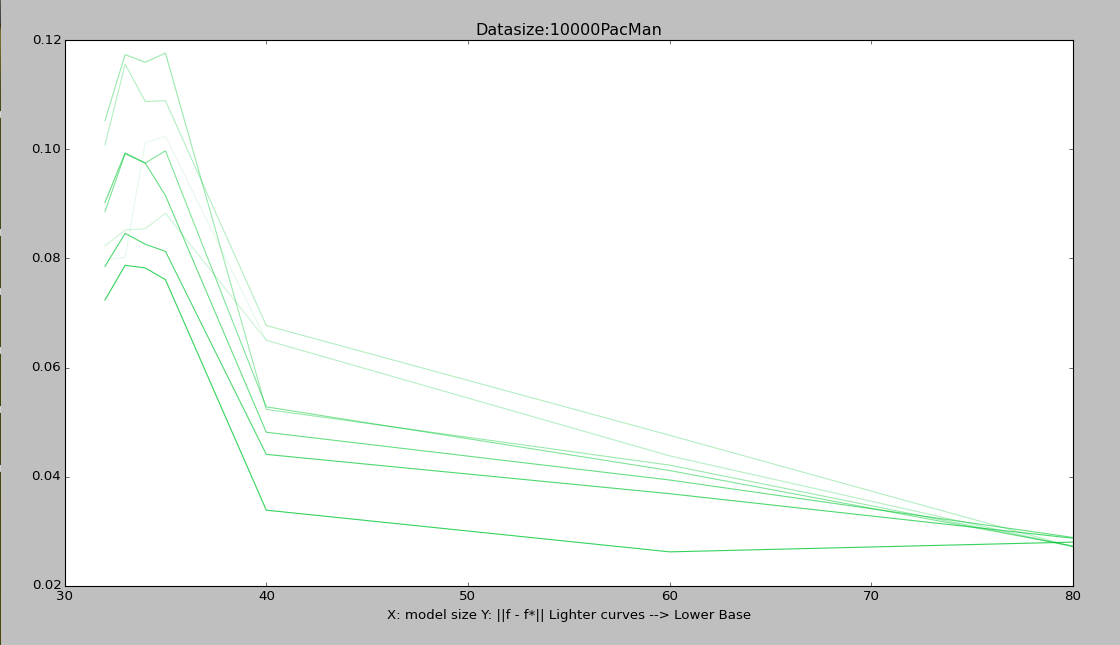
\includegraphics[width=60mm]{lucasplots/pacman10000.png}
\caption{Timing predictions in Pacman \label{overflow}}
\end{figure}


\begin{figure}[ht!]
\centering
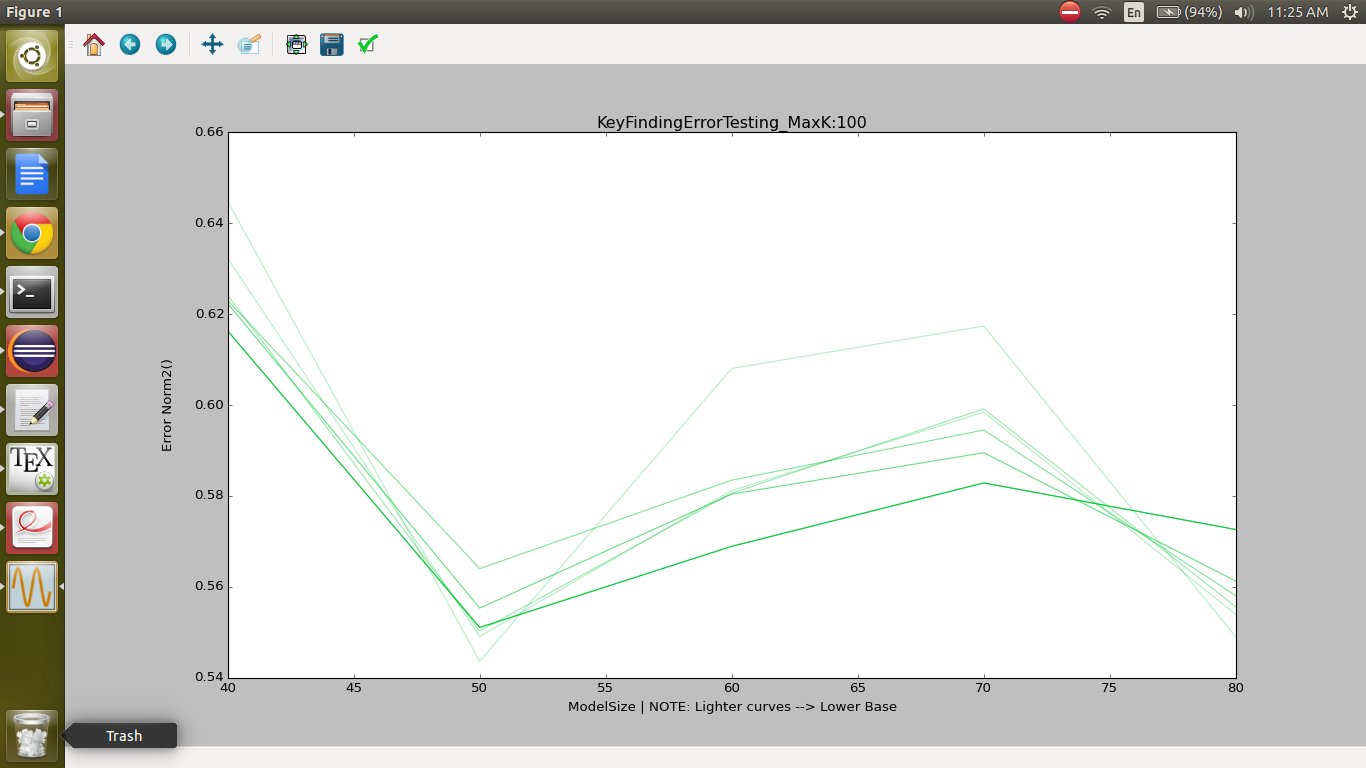
\includegraphics[width=60mm]{lucasplots/Distances.png}
\caption{Distance predictons from key \label{overflow}}
\end{figure}

Here, the Base System outperforms the naive by 100\% for timing and 45\% for distances.

\subsection{Multiple Observations}

Next, we change our set of observations to wall colors of the labyrinth. 

\begin{figure}[ht!]
\centering
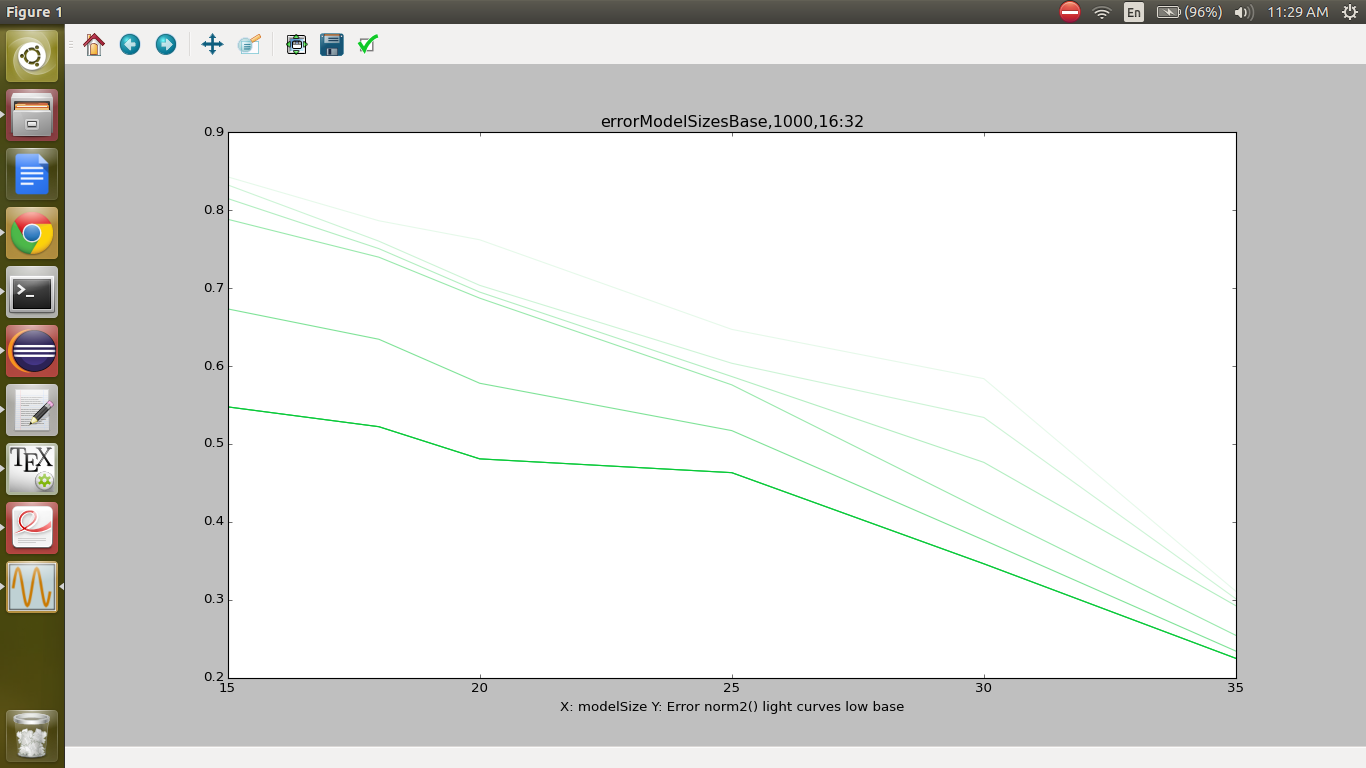
\includegraphics[width=60mm]{lucasplots/MO:16,32.png}
\caption{Predicting wall colors \label{overflow}}
\end{figure}

Here, the Base System outperforms that naive approach by 55\%. For this environment, we construct the Base System separately for each symbol. In general, one might want to use a custom heuristic to optimize the construction.

%Cite figures

\section{Relevance and Future Work}
The spectral framework for learning in partially observable environments has better theoretical guarantees \cite{Lamport:LaTeX} than non-spectral methods. In this work, we showed a way to significantly improve results when one wants a smaller model of the environment as often occurs in practice. In future work, we hope to see a theoretical analysis of the apparent improvement of the Base System and further optimization of it's construction.
\begin{comment}
This is \textit{italic}, \textbf{bold}, \textsc{small caps}, \textsf{sans serif}

Math is writen inside dollars: $a = b$, $a_k$, $b^s$, $a_k^j$, $a_{opt}^{\star}$ $\sin(2 \pi) = 0$, greek letters are intuitive $\alpha$, $\beta$, $\sigma$, $\Sigma$, $\Gamma$, and so on

Full line equations use 2 dollars
$$ \sum_{i=0}^{\infty} \gamma^i = \frac{1}{1-\gamma} $$

Other math symbols $a \in A \cap B \subseteq C \equiv X \sim Y \leq Z$
\end{comment}

%
% The following two commands are all you need in the
% initial runs of your .tex file to
% produce the bibliography for the citations in your paper.
\bibliographystyle{abbrv}
\bibliography{sigproc}  % sigproc.bib is the name of the Bibliography in this case
% You must have a proper ".bib" file
%  and remember to run:
% latex bibtex latex latex
% to resolve all references
%
% ACM needs 'a single self-contained file'!
%.
\subsection{References}
Generated by bibtex from your ~.bib file.  Run latex,
then bibtex, then latex twice (to resolve references)
to create the ~.bbl file.  Insert that ~.bbl file into
the .tex source file and comment out
the command \texttt{{\char'134}thebibliography}.

\end{document}



